\documentclass[12pt]{article}
\usepackage[tmargin=1.5in]{geometry}
\usepackage{relsize}
\usepackage{babel}
\usepackage{listings}
\usepackage{amsmath}
\usepackage{amssymb}
\usepackage[table]{xcolor}
\usepackage[pdftex]{graphicx}
\usepackage{caption}

\setlength{\parindent}{0cm}  % Indentation prohibited by default

\title{Aufgabenblatt 8: MPI-Jacobi-Hybrid-Leistungsanalyse}
\author{Gruppe: CaesarBaurMueller}
\date{\today}

\begin{document}
\maketitle

\begin{sloppypar}
\section*{Leistungsanalyse}
Im Folgenden haben wir die Runtimes der verschiedenen Aufrufe des hybriden OpenMP-MPI-Programms dargestellt. Alle Werte sind in Sekunden angegeben.

\begin{table}[ht]
    \caption{Leistungsanalyse der hybriden Jacobi-MPI-Implementierung auf den Nodes \textit{west1}, \textit{west3} und \textit{west4}}
    \begin{tabular}{l|ccc|c}
        Parameters & Runtime 1 & Runtime 2 & Runtime 3 & Average \\ \hline
        12 Processes, 1 Thread & 35.875082 & 35.678267 & 35.760198 & 35.771182 \\ 
        24 Processes, 1 Thread & 31.245743 & 30.489378 & 30.935176 & 30.890099 \\ 
        1 Processes, 12 Threads & 418.689716 & 418.769830 & 418.814418 & 418.757988 \\ 
        1 Process, 24 Threads & 420.622928 & 418.811581 & 418.805169 & 419.413225 \\ 
        2 Process, 6 Threads & 207.886090 & 208.154691 & 208.584383 & 208.208388 \\ 
        2 Processes, 12 Threads & 207.843282 & 210.080138 & 207.777904 & 208.567108 \\ 
        12 Processes, 2 Threads & 36.321066 & 35.980709 & 36.190474 & 36.164083 \\ 
    \end{tabular}
\end{table}

Eine andere graphische Darstellung findet sich in der folgenden Grafik:
\begin{figure}[ht]
    \centering
    \caption{Leistungsanalyse der hybriden Jacobi-MPI-Implementierung auf den Nodes \textit{west1}, \textit{west3} und \textit{west4}}
    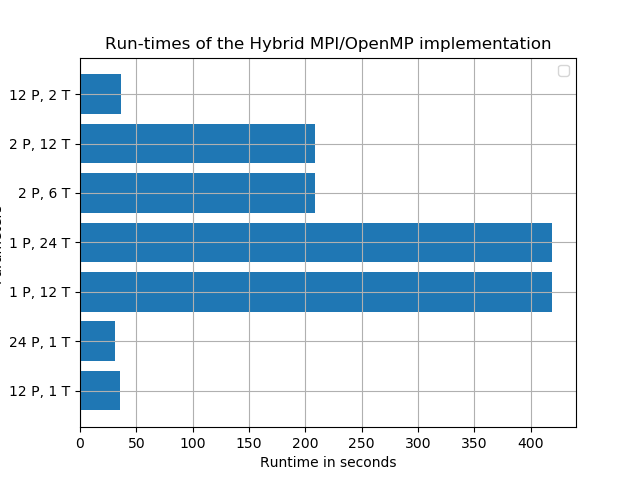
\includegraphics[width=0.8\textwidth]{average-plot-hybrid-mpi-omp.png}
\end{figure}
\newpage

Wir können aus den Ergebnissen ableiten, dass unsere OpenMP-Parallelisierung vermutlich nicht richtig funktioniert. Die MPI-Parallelisierung hingegen schon. Falls die OpenMP Parallelisierung funktionieren ordnungsgemäß funktionieren würde, würde dies bedeuten dass OpenMP im Zusammenspiel mit MPI unwirksam würde. Erkennbar ist dies aus den nahezu identischen Laufzeiten der OpenMP-Runtimes mit den (hier nicht aufgeführten) sequentiellen Ergebnissen (ca. $418s$). \\

Die MPI-Parallelisierung hingegen funktioniert gut und erreicht einen Speedup von ca. $14$ mit 24 Prozessen.

\end{sloppypar}
\end{document}